\documentclass{article}
% General document formatting
\usepackage[margin=0.7in]{geometry}
\usepackage[parfill]{parskip}
\usepackage[utf8]{inputenc}
\usepackage{graphicx}
\usepackage{hyperref}
\usepackage{adjustbox}
\usepackage[backend=biber, style=ieee]{biblatex}
\addbibresource{citations.bib}
\usepackage[nomain,acronym,xindy,toc]{glossaries} % nomain, if you define glossaries in a file, and you use \include{INP-00-glossary}
\makeglossaries
\usepackage[table,xcdraw]{xcolor}
\usepackage{appendix}
\usepackage{gensymb}
\usepackage{wrapfig}
\hypersetup{
    colorlinks,
    citecolor=black,
    filecolor=black,
    linkcolor=black,
    urlcolor=black
}
\graphicspath{ {./images/} }

\input{glossary}
    

\begin{document}
    \title{Simple Solar Power}
    \author{Christopher Molina, Colter Roche, Damien Kent, David Rodriguez, Halle Fortune}
    \date{\today}
    \maketitle
    \newpage

    \pagenumbering{roman}
    \tableofcontents
    \listoffigures
    \printglossary[type=\acronymtype]
    \newpage
    \pagenumbering{arabic}

    \section{Introduction}
        Solar concentration is the technique of using mirrors, reflective material, or lenses to focus large 
        amounts of sunlight on to a smaller area. Using this process allows for potentially enormous amounts of heat 
        to be produced. This process would be necessary in a situation without a means to provide power, healthy 
        consumption of food, and hot or clean water. It is a perfect alternative to creating a basic fire because 
        adequate fire wood is not always available but sunlight is an unlimited resource. Construction of a device 
        using this system will help in providing the community with a sustainable long term heating or cooking method 
        that does not require electricity or fire. The device that this manual will be discussing is a Parabolic 
        Dish Solar Concentrator (PDSC) focused on the application for cooking food and boiling water. The PDSC is a 
        concentrator that is in the shape of a satellite dish that provides a central point for the sunlight to heat. 
        \begin{wrapfigure}{r}{0.4\textwidth}
            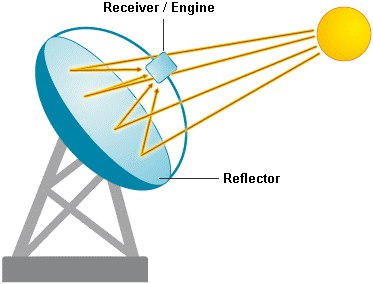
\includegraphics[scale=.5]{Concentrator-diagram}
            \caption{Reflection of sunlight to the focal point\cite{Reflector}}
        \end{wrapfigure}

        \subsection{Background}
            Solar concentration was first used for cooking as early as 1767.  Parabolic Dish Solar Collectors were first developed 
            as a source of power generation in the early part of the industrial revolution, born from fears that Europe would run 
            out of coal.  Through the use of curved mirrors, sunlight can be concentrated into a point, generating intense heat.  
            This heat can then be used to boil water, produce steam, cook food, and generate power.  The P.D.S.C described in this 
            manual can generate temperatures of close to 200 degrees F, and can be used anywhere a direct source of sunlight is 
            available, including high altitudes.
        
    
    \section{Materials, Tools and Skills}
        \subsection{Materials Required}
            \begin{table}[h]
                \begin{tabular}{|p{3cm}|p{3cm}|p{11cm}|}
                \hline
                \rowcolor[HTML]{C0C0C0} 
                Item                                                        & Amount                & Notes                                                                                                                \\ \hline
                1/2-inch plywood                                            & Varies                & For the Panel Template.  If Jigsaw not available for cutting, heavy duty cardboard may be substituted.               \\ \hline
                1x4 boards                                                  &                       & For the Panel Template.                                                                                              \\ \hline
                Square Sheet of paper                                       & 1                     & Used to measure the angle for the Panel Template.  Alternatively, a protractor may be used                           \\ \hline
                Heavy duty cardboard                                        &                       & Corrugated cardboard is ideal.                                                                                       \\ \hline
                Adhesive                                                    &                       & Spray adhesive works the best.  Alternatively, glue can be used instead.                                             \\ \hline
                Aluminum foil                                               & Enough to cover dish. & Must be reflective.  Heavy duty works best.                                                                          \\ \hline
                Metal strip                                                 &                       & Reinforces the Dish, and attaches it to the Frame.  Drywall corner strips work well, if available.                   \\ \hline
                1-inch 8-32 screws with flat washers and nuts               &                       &                                                                                                                      \\ \hline
                6-inch 1/4-20 carriage bolt with flat washers and wing nuts &                       & Holds the center of the Dish, and serves as the guide for alignment with the Sun.  Threaded rod may be used instead. \\ \hline
                2x4s                                                        &                       & Used for the base                                                                                                    \\ \hline
                3-inch deck screws                                          &                       &                                                                                                                      \\ \hline
                1/2-inch electrical conduit                                 &                       & If not available, metal rods can be used instead.                                                                    \\ \hline
                Grill grate                                                 & 1                     & Holds the cooking pot.                                                                                               \\ \hline
                Binding wire                                                &                       & Holds the grate                                                                                                      \\ \hline
                \end{tabular}
            \end{table}
        \newpage
        \subsection{Tools Required}
            \begin{table}[h!]
                \begin{tabular}{|p{3cm}|p{14cm}|}
                \hline
                \rowcolor[HTML]{C0C0C0} 
                Tool                 & Notes                                                                                                           \\ \hline
                T Square             & For drawing the parabola required for the dish template.  See appendix A                                        \\ \hline
                550 Cord             & For drawing the parabola required for the dish template.  See appendix A                                        \\ \hline
                Pencil               &                                                                                                                 \\ \hline
                Clamps               &                                                                                                                 \\ \hline
                Measuring Tape       &                                                                                                                 \\ \hline
                Duct Tape            & Must be heavy duty                                                                                              \\ \hline
                Utility Knife        &                                                                                                                 \\ \hline
                Scissors             &                                                                                                                 \\ \hline
                Jigsaw               & Jigsaw is ideal for cutting template panels.  In case power not available, different materials may be required. \\ \hline
                Drill and Drill Bits & Used for building frame.  Heavy duty adhesive or other fastening methods may be substituted.                    \\ \hline
                Hammer               &                                                                                                                 \\ \hline
                \end{tabular}
                \end{table}
        
    \section{P.D.S.C. Saftey Guidelines}
        To mininmize the risk of injury when using the P.D.S.C., please follow the safety guidelines listed below, and throughout the manual.
        \begin{enumerate}
            \item Do not use the P.D.S.C. on cloudy or very cold days, to minimize the risk of foodborne illnesses.
            \item Always use a thermometer to check the internal temperature of food before eating it, if possible.
            \item Wear protective eyeware, and avoid looking directly into the dish during use, to prevent eye damage.
            \item The P.D.S.C. may become very hot, especially near the cooking area.  Always wear protective gloves to prevent burns.
            \item Keep children and pets away from the P.D.S.C. when in use.
        \end{enumerate}
    \section{Preparing the Location}
        \subsection{Environmental Specifications}
        The P.D.S.C. is well suited to cooking at high altitudes and only requires
        a direct view of the sun to function.  
        
        Do not try to use the P.D.S.C. to cook food 
        on overcast days, at risk of not heating the food to a safe temperature. 
        Make sure to clear the area of any obstruction and make sure that the P.D.S.C. Frame is 
        on a stable, level surface.

    \section{Building the P.D.S.C.}
        While following this guide, keep in mind that this design can be built
        larger or smaller depending on how much material is available.  The measurements listed
        in diagrams and in the instructions are one possible size of reflector. 
        
        \subsection{Building the P.D.S.C. Dish Template}
        In order to easily make the panels for the P.D.S.C., a template is required.  See appendix A for instructions
        on drawing a parabola using string and a ruler or T-square.  The more sections the dish has,
        the more efficiently the P.D.S.C. will function.  The instructions below are designed for 16 sections,
        but the angle can be ajusted to allow for more or less sections.
            \begin{enumerate}
                \item For the template, take a piece of plywood slightly longer than the desired panel length, and about 2/3rds as long
                \item Measure 8 in. from one end on the long side of the plywood piece. This is the focal point of the parabola. Mark the focal point clearly.
                \item See Appendix A for steps to use the focal point, rope, pencil, and T-square to draw a parabolic arc on the plywood.
                \item Once the parabola has been marked, measure from the focal point to the arc of the parabola.  This is the focal length.  Make a note of this measurement.
                \item Draw a line along the focal length, and then cut out the marked area. Use this piece to cut a second, matching piece. These parts will make up the sides of the template.
                \item The angle required for 16 sections is 22.5\degree. To measure this angle, fold the square piece of paper corner to corner to get a 45\degree angle. Then, fold in half again for a 22.5\degree angle.
                \item Use the paper reference to form the correct angle at the apex of the plywood form, then measure the wide end.
                \item Cut a piece of 1x4 board to match the measured length of the wide end.  Secure the boards to the wide end with tape to reinforce the plywood.
                \begin{figure}[!htb]
                    \minipage{0.32\textwidth}
                      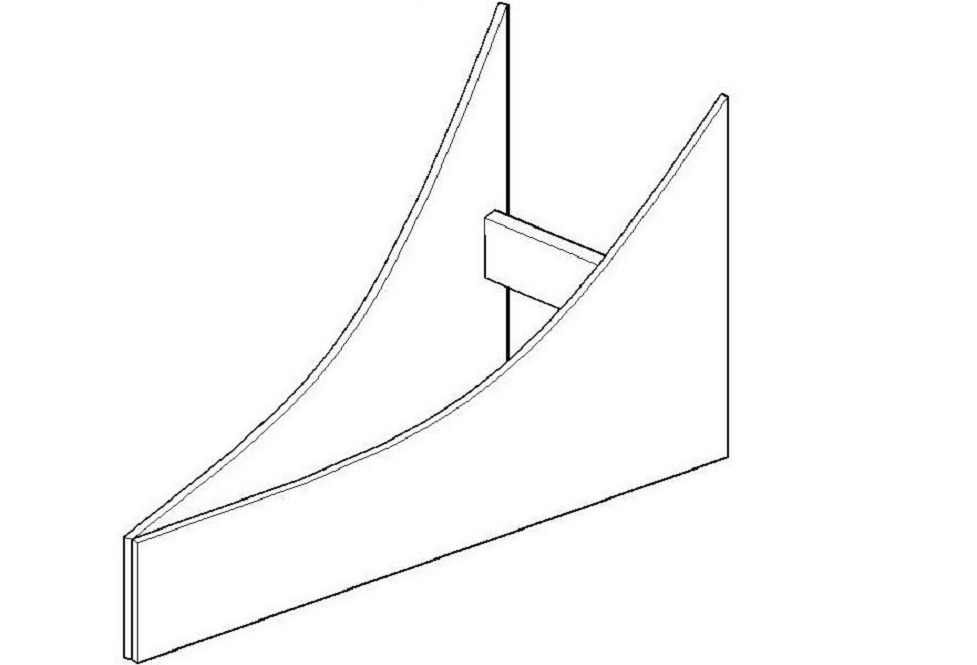
\includegraphics[width=\linewidth]{template_3d}
                      \caption{Isometric Diagram of completed template form}\label{fig:awesome_image1}
                    \endminipage\hfill
                    \minipage{0.32\textwidth}
                      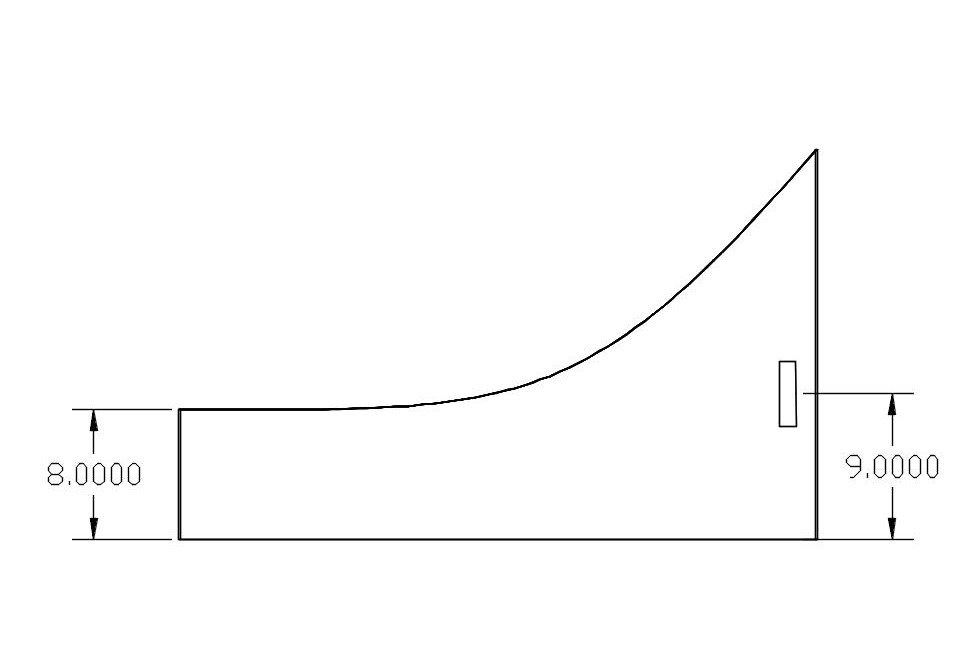
\includegraphics[width=\linewidth]{template_side}
                      \caption{Side view of template form with sample measurments.}\label{fig:awesome_image2}
                    \endminipage\hfill
                    \minipage{0.32\textwidth}%
                      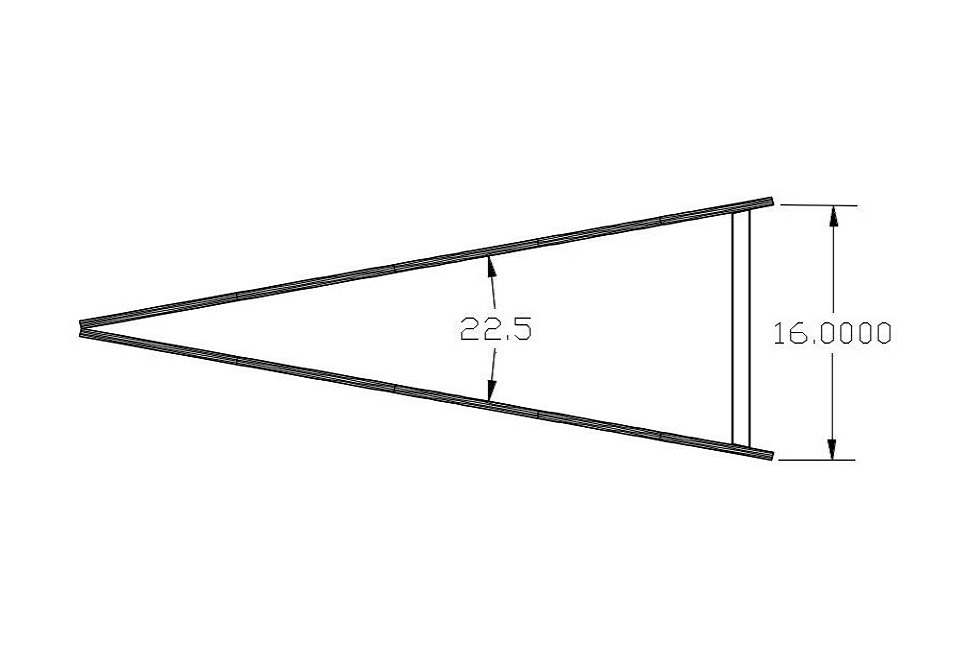
\includegraphics[width=\linewidth]{template_top}
                      \caption{Top view of template form with sample measurements}\label{fig:awesome_image3}
                    \endminipage
                \end{figure}
                \item Clamp a piece of cardboard the the plywood form and mark along the edges of the form, against the cardboard.
                \item Cut out the cardboard along the lines drawn. The cardboard section is the template for all the sections of the dish.

            \end{enumerate}
            
        \subsection{Building the P.D.S.C. Dish}
            The P.D.S.C. Dish is made from 16 sections of aluminum foil coated cardboard made into a dish shape. The template made in the previous 
            section is used to make the individual parts, which are then assembled.
            \begin{enumerate}
                \item Use the P.D.S.C. template made in the previous step to cut 15 more sections, for a total of 16 identical sections.
                \item Crease each section every 2 inches starting from the wide end.
                \item Once all the sections have been creased, the aluminum foil needs to be applied.  Make sure the shiny side of the aluminum is facing out when covering the sections. Spray adhesive is recommended, but if that is not available, a thin layer of liquid glue will work.  The panels need to be as smooth and shiny as possible.
                \item Leave enough foil to fold over the edges and glue to the back of the panels.
                \item Tape the panels together using heavy duty duct tape.  Use something to support the center of the dish when assembling the sections.
                \item If using a drywall corner strip to support the dish, hammer it flat.
                \item Drill holes in the ends of the metal strip and tape the strip to the back of the dish.  The holes are used to attach the P.D.S.C. dish to the frame.
                \item Screw the edge of the dish to the edge of the metal strip using the 1-inch 8-32 screws with flat washers and nuts.
                \item Cut a 12 inch circle of cardboard and cover with aluminum foil.
                \item Drill or cut a hole in the center of the cardboard circle and bolt a 6-inch 1/4-20 carriage bolt with flat washers and wing nuts to the center of the circle.  The long end should point towards the focal point of the P.D.S.C. Dish Assembly.
                \item Attach the cardboard circle to the center of the Dish assembly.  The long part of the center screw will serve as a guide for aligning the dish with the Sun.
                \item The P.D.S.C. Dish Assembly is now complete. 
                
            \end{enumerate}
    
        \subsection{Building the P.D.S.C. Frame}
            The P.D.S.C. Frame is a simple structure built from 2x4 boards.  The P.D.S.C. Dish Assembly attaches to the Frame using the metal support strip and 2 6-inch 1/4-20 carriage bolts with flat washers and wing nuts.  Measurments in the following diagrams are suggestions, and can be easily adjusted to fit the diameter of the completed P.D.S.C Dish Assembly.
            \begin{enumerate}
                \item Measure the diameter of the P.D.S.C. Dish assembly. The frame consists of 2 T-shaped reinforced end pieces and a 2x4 board holing them together.
                \item The T-shaped end pieces need to be nearly as tall as the diameter of the dish, and the board holding the 2 ends together must be as long as the diameter of the dish.
            \end{enumerate}
            \begin{figure}[!htb]
                \minipage{0.32\textwidth}
                  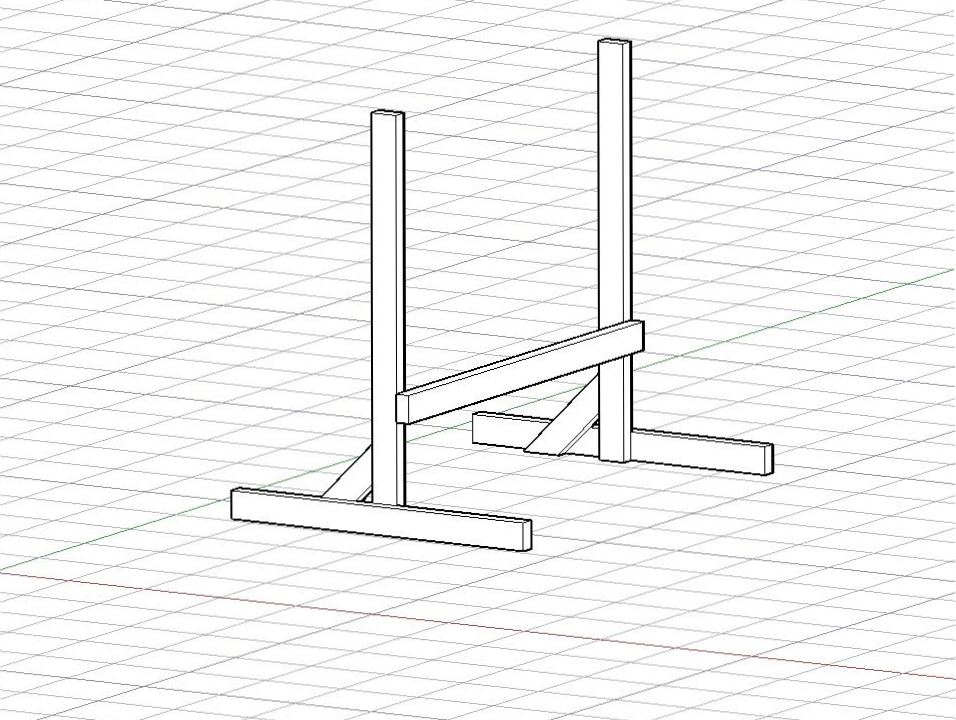
\includegraphics[width=\linewidth]{base_3d}
                  \caption{Isometric Diagram of completed base}\label{fig:awesome_image1}
                \endminipage\hfill
                \minipage{0.32\textwidth}
                  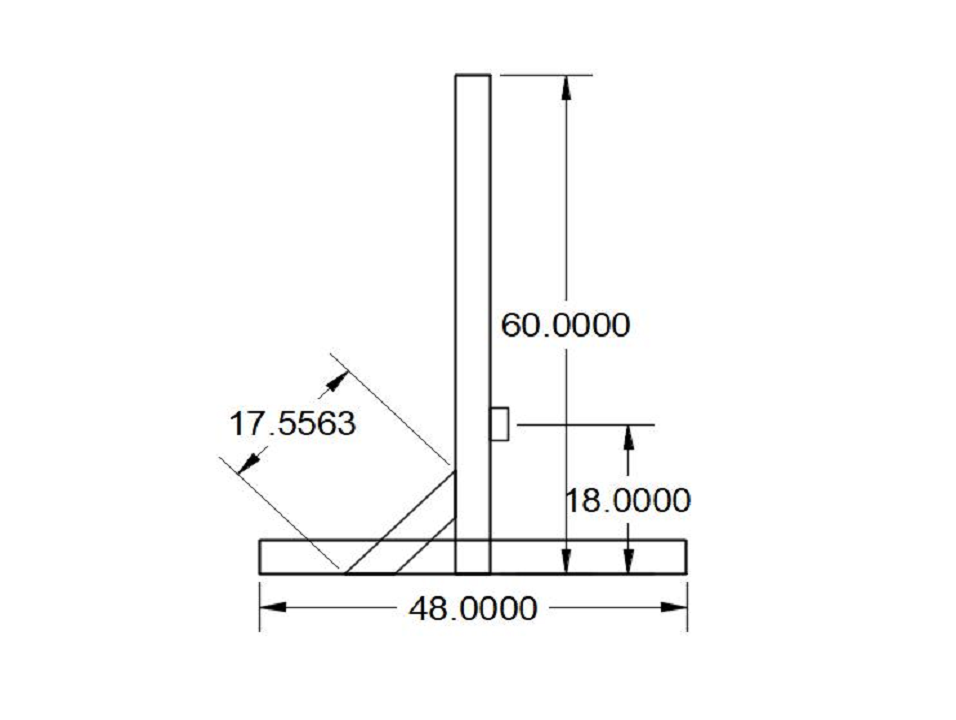
\includegraphics[width=\linewidth]{base_side}
                  \caption{Side view of base with sample measurments}\label{fig:awesome_image2}
                \endminipage\hfill
                \minipage{0.32\textwidth}%
                  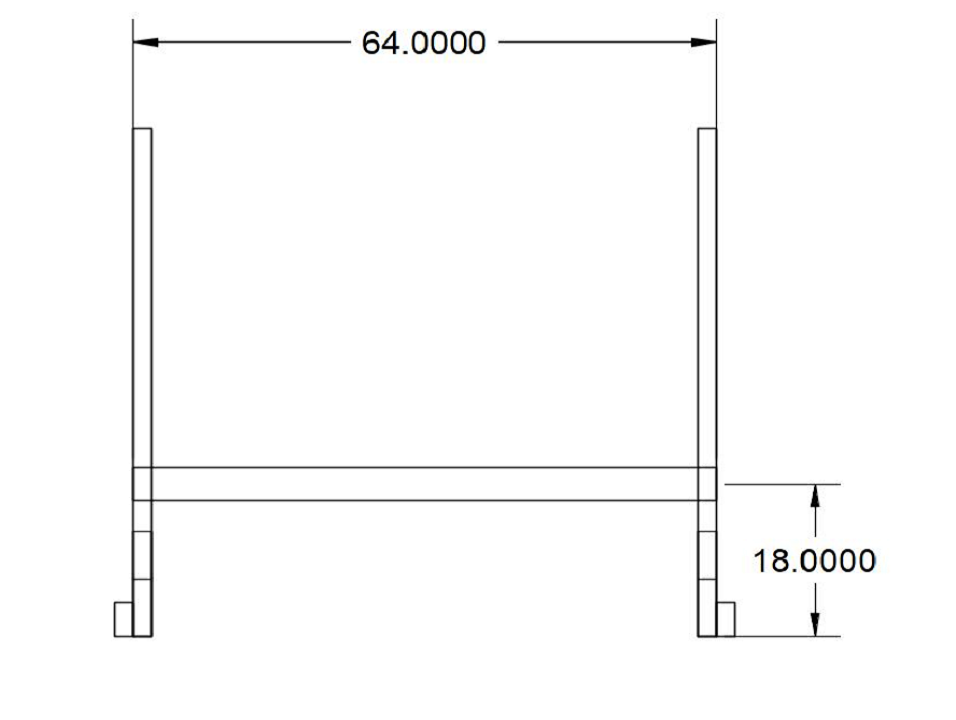
\includegraphics[width=\linewidth]{base_rear}
                  \caption{Rear view of base with sample measurements}\label{fig:awesome_image3}
                \endminipage
                
                \end{figure}
        \subsection{Assembling the P.D.S.C.}
            Assembly and usage of the P.D.S.C. is fairly simple. A wooden dowel or section of metal rod can be used the hold the 
            \begin{enumerate}
                \item Drill a hole in each upright part of the frame, a distance half the diameter of the P.D.S.C. Dish from the bottom.
                \item Use 2 6-inch 1/4-20 carriage bolt with flat washers and wing nuts to attach the metal strip on the dish to the stand using the holes drilled in the previous step.
                \item Make sure the dish is firmly bolted to the stand, but is still able to be rotated.
                \item Measure from the ground to the previously noted focal point of the dish.  This is the height at which the grill grate needs to be mounted for optimal heat production.
                \item Mount 2 lengths of the 1/2 inch electrical conduit using clamps to the Frame at the same height as the focal point.
                \item Attach the grill grate to the conduit using binding wire.  This is where the pan will go when the P.D.S.C. is in use.
                \item Adjust the P.D.S.C. Dish assembly to the correct angle, and use a wooden dowel and clamp to hold the dish in position.
            \end{enumerate}
            The P.D.S.C. is now complete and ready for use.
    \newpage
    \section{P.D.S.C. Operation}
        The P.D.S.C. has a variety of uses, due to it's ability to produce heat without combustion.  For best results, use a dark colored pot or pan to cook with.
        Follow the steps below to safely use the P.D.S.C. for food saftey purposes.

        \subsection{Cooking food}
        When cooking food, especially meat or fish, with the P.D.S.C. it is extremely important that the food reach an internal temperature of 165\degree F.  Failure to reach these temperatures
        may result in the contraction of food borne illnesses.
            \begin{enumerate}
                \item Make sure the area is clear of obstructions, that the sky is clear of clouds, and that there are at least 2 hours of direct sunlight available.
                \item Position the P.D.S.C. Dish assembly facing the sun, using the large screw at the center of the dish as a guide.  If the shadow is not visible, then the dish is properly aligned with the Sun.
                \item Place the food to be cooked in a dark colored pan (cast iron should be fine), and place on the rack.
                \item Depending on the food type, it may help to wrap the pan in a clear plastic bag to seal in some of the heat and moisture.
                \item The P.D.S.C. Dish Assembly will need to be rotated every 5-10 minutes to ensure optimal heating.
                \item Use a thermometer, if available, to check the internal temperature has reached 165\degree.  If a thermometer is not available, make sure the food is thoroughly cooked.
                \item Average cooking time depends on what kind of meal is getting prepared.
            \end{enumerate}
        \subsection{Pasturizing water}
        The steps to pasturize water to make it safe for drinking are very similar to the steps above, with some minor differences.
        The major differences are listed below.
            \begin{enumerate}
                \item The temperature required to pasturize water is 149\degree F.
                \item The water must be brought to at least this temperature for 6-8 minutes.
                \item After that time, the water will be safe to drink.
            \end{enumerate}
    \section{Maintainance and Troubleshooting}
        Compared to heating systems reliant on combustible fuel, the P.D.S.C. requires very little maintainance. For optimal performance, however, some level of care should be taken.
        \subsection{Maintanaince}    
            Follow the steps below to ensure the P.D.S.C. is not damaged during use.
                \begin{enumerate}
                    \item If any spills occur on the reflective material be sure to clean it up immediately after cooking, as staining the reflective material may reduce the solar cooker’s effectiveness.
                    \item Make sure to clean the reflective material every so often with a dry or wet cloth so as to keep the solar cooker at maximum efficiency (If using a wet cloth make sure to dry it with a dry cloth afterwards).
                    \item Bring in the solar cooker if you are expecting rain or it starts raining. The water can damage the cardboard/wood as well as the reflective material of your solar cooker.
                    \item Beware of strong winds as they might knock the solar cooker over and damage it. Make sure that the P.D.S.C. is secured outside.

                \end{enumerate}
        \subsection{Troubleshooting}
            If the P.D.S.C. does not seem to be working properly, follow the steps below to fix the issue.
            \begin{enumerate}
                \item Check to make sure the P.D.S.C. has an unobtructed view of the sun.
                \item Check the alignment of the P.D.S.C. Dish assembly.  If the guide rod has a shadow visible, adjust the angle as necessary.
                \item Make sure that the reflective surface is clean and free of debris.
                \item Check that the cooking surface is at the correct height. If a piece of paper is placed on the cooking surface, the light should be concentrated in a single spot.
            \end{enumerate}
    \section{Additional Use Cases}
    The P.D.S.C. can be adapted for large scale useage including the folowing examples.
        \subsection{Heating Water}
            The larger the P.D.S.C. Dish is, the higher the possible temperature generated is.  With a sufficiently large dish, or a parabolic trough system,
            water can be heated on a large scale, allowing for use for bathing and cleaning of laundry.
            \begin{figure}[h]
                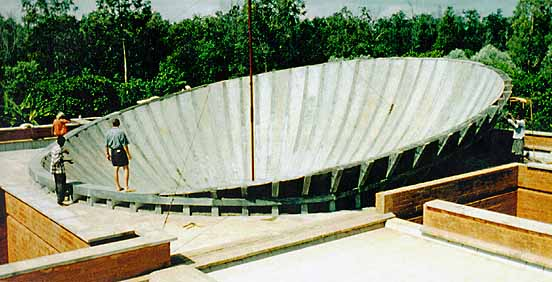
\includegraphics[scale=.5]{large_dish}
                \caption{Large scale parabolic dish collector}
            \end{figure}
        \subsection{Steam Generation}
            On a large enough scale, the P.D.S.C. should be able to produce steam from water.  This would allow for the production of electricity via a steam turbine generator,
            or a stirling engine placed at the focal point of the dish assembly.
            \begin{figure}[h]
                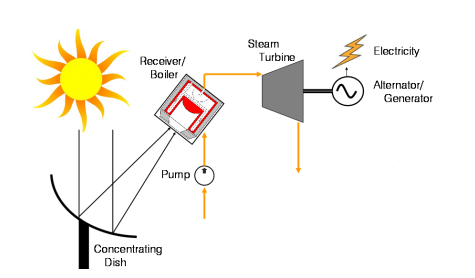
\includegraphics[scale=.75]{steam_power}
                \caption{System diagram for steam turbine setup.\cite{Steam-Gen}}
            \end{figure}
        \subsection{Under-floor Heating}
            If heated water was produced in larger amounts, with some degree of storage, then hot water could be run through 
            pipes underneath the floor.  This would provide heating for the floor, and by extension, the room.
            \begin{figure}[h]
                \minipage{0.48\textwidth}
                  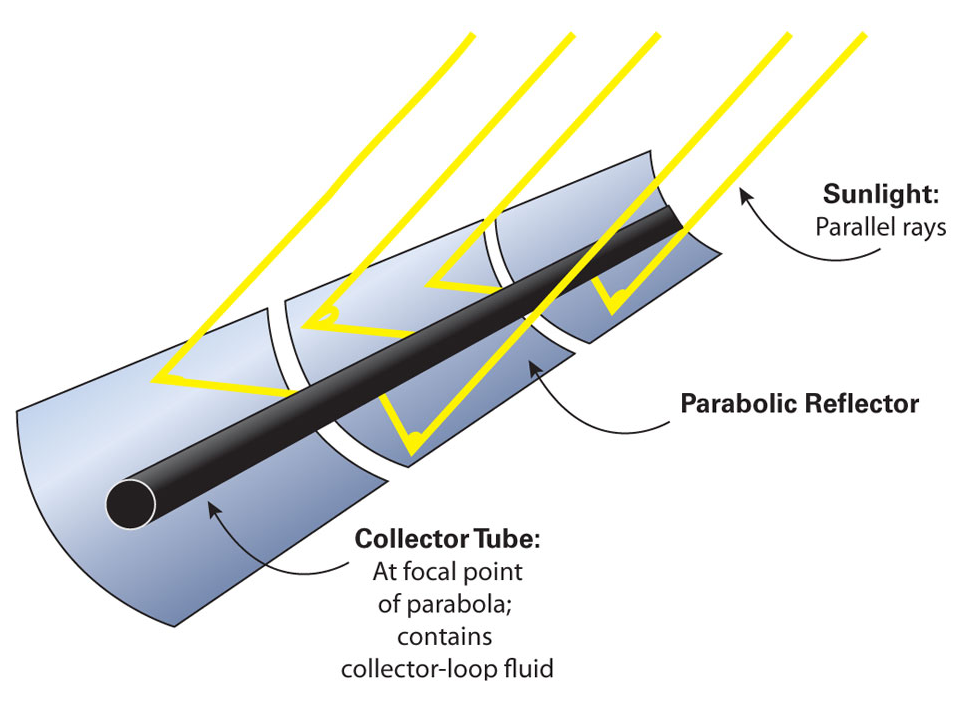
\includegraphics[width=\linewidth]{trough}
                  \caption{Example layout for trough collector system.\cite{Trough-Gen}}
                \endminipage\hfill
                \minipage{0.48\textwidth}
                  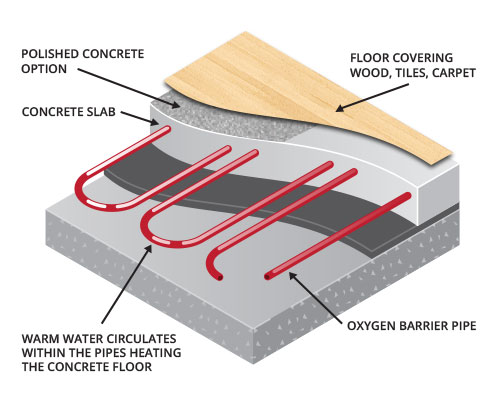
\includegraphics[width=\linewidth]{underfloor}
                  \caption{Cross-section of flooring setup with radian heating pipes.}
                \endminipage\hfill
            \end{figure}
    \appendix
    \newpage
    \appendixpage
    \addappheadtotoc
    \section{Drawing a Parabola}
        In order to efficiently concentrate solar energy, a parabolic dish or trough is required.  The following intructions describe a simple method of drawing a parabolic curve.\cite{Parabola}
        \begin{enumerate}
            \item \begin{minipage}[t]{\linewidth}
                \raggedright
                \adjustbox{valign=t}{%
                  
\includegraphics[scale=1]{parabola01}% 
                }
      
                \medskip
                Mark the focal point on the surface the parabola is to be drawn on.
            \end{minipage}
            \item \begin{minipage}[t]{\linewidth}
            \raggedright
            \adjustbox{valign=t}{%
              
\includegraphics[scale=1]{parabola02}% 
            }
  
            \medskip
            Align a T-square or straight edge with the marked focal point.
            \end{minipage}
            \item \begin{minipage}[t]{\linewidth}
                \raggedright
                \adjustbox{valign=t}{%
                
\includegraphics[scale=1]{parabola04}% 
                }

                \medskip
                Attach a rope or string to the focal point and the top of the t-square using tacks or nails, as shown above.
            \end{minipage}
            \item \begin{minipage}[t]{\linewidth}
                \raggedright
                \adjustbox{valign=t}{%
                
\includegraphics[scale=1]{parabola06}% 
                }

                \medskip
                Place a pen or pencil at the bottom of the t-square in the rope, and slowly slide the t-square away from the focal point, 
                holding the pen against the t-square.  
                \end{minipage}
            \item \begin{minipage}[t]{\linewidth}
                \raggedright
                \adjustbox{valign=t}{%
                
\includegraphics[scale=1]{parabola07}% 
                }

                \medskip
                Continue sliding the t-square, forming a smooth curve.  The resulting curve is half of a parabola.
            \end{minipage}
            \item \begin{minipage}[t]{\linewidth}
                \raggedright
                \adjustbox{valign=t}{%
                
\includegraphics[scale=1]{parabola08}% 
                }

                \medskip
                The completed curve.
            \end{minipage}
        \end{enumerate}
    \newpage
    \printglossary
    \printbibliography
\end{document}